\section{Firepolet massespektrometer}
Det firepolede massespektrometer bruger stabiliteten af ionernes bane i et oscillerende elektrisk felt til at separere dem afhængig af deres $m/z$ \parencite{massspec}.
Den består af fire cirkulære, eller ideelt hyperbolske, parallelle stænger, som kan ses på \cref{fig:quadpole}.
\begin{figure}[H]
	\centering
	\begin{subfigure}{.6\linewidth}
		\centering
		\tikzset{rod/.style={cylinder, draw, shape aspect=.5,
					cylinder uses custom fill, cylinder end fill=black!50,
					minimum height=60,
					cylinder body fill=black!20,
					scale=2, rotate=200,anchor=east}
		}
		\begin{tikzpicture}
			% Rod bottom + left
			\node[rod] (rb) at (0,-0.5,0) {}; % bottom
			\node[rod] (rl) at (-0.5,0,-0.5) {}; % left
			% Beam
			\draw[red,arrows = {-Stealth},rotate=20] (-1,0) node[black,anchor=north,rotate=20] {Ionkilde} -- (0,0) sin +(.2,.2) cos +(.2,-.2) sin +(.2,-.2) cos +(.2,.2) sin +(.2,.2) cos +(.2,-.2) sin +(.2,-.2) cos +(.2,.2) sin +(.2,.2) cos +(.2,-.2) sin +(.2,-.2) cos +(.2,.2) sin +(.2,.2) cos +(.2,-.2) sin +(.2,-.2) cos +(.2,.2) sin +(.2,.2) cos +(.2,-.2) sin +(.2,-.2) cos +(.2,.2) sin +(.2,.2) cos +(.2,-.2) -- +(1,0) node[black,anchor=south,rotate=20] {Detektor};
			% Rod top
			\node[rod] (rt) at (0,0.5,0) {}; % top
			% Rod see through
			\node[rod,minimum height=6] (rr1) at (0.5,0,0.5) {}; % right 1
			\node[rod,minimum height=6,xshift=-50,cylinder end fill=black!20] (rr2) at (0.5,0,0.5) {}; % right 2
			\draw[dashed] (rr1.after bottom) -- (rr2.before top);
			\draw[dashed] (rr1.before bottom) -- (rr2.after top);
			% Firpol text
			\node[anchor=south,yshift=15,rotate=20] at (rt.north east) {Firpol};
		\end{tikzpicture}
		\caption{Diagram over firpol. Den røde bane viser banen af et stabilt molekyle, som altså har den rette $m/z$.}
		\label{fig:quadpolebig}
	\end{subfigure}\hspace{.05\linewidth}%
	\begin{subfigure}{.3\linewidth}
		\centering
		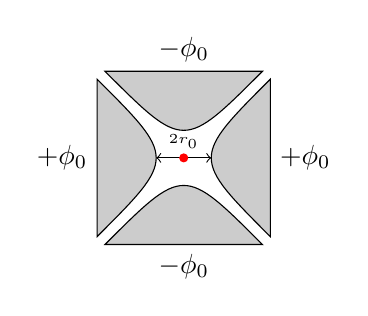
\begin{tikzpicture}
			\draw[fill=black!20] (-1,1.1) .. controls (0,.1) .. (1,1.1) -- cycle;
			\draw[fill=black!20] (-1,-1.1) .. controls (0,-.1) .. (,-1.1) -- cycle;
			\begin{scope}[rotate=90]
				\draw[fill=black!20] (-1,1.1) .. controls (0,.1) .. (1,1.1) -- cycle;
				\draw[fill=black!20] (-1,-1.1) .. controls (0,-.1) .. (1,-1.1) -- cycle;
			\end{scope}

			\node[anchor=south] at (0,1.1) {$-\phi_0$};
			\node[anchor=north] at (0,-1.1) {$-\phi_0$};
			\node[anchor=east] at (-1.1,0) {$+\phi_0$};
			\node[anchor=west] at (1.1,0) {$+\phi_0$};

			\draw[<->] (-.35,0) -- (0,0) node[anchor=south] {\tiny$2r_0$} -- (.35,0) ;

			\filldraw[red] (0,0) circle (0.05);
		\end{tikzpicture}
		\caption{Snit af firpol, med potentialerne $\phi_0 = U - V \cos{\omega t}$.}
		\label{fig:quadpolecharge}
	\end{subfigure}
	\caption{Diagram over firpolet MS, med snit som viser potentialerne i stængerne. \parencite{massspec}}
	\label{fig:quadpole}
\end{figure}

Det elektriske potentiale i stængerne som ses på \cref{fig:quadpolecharge} er givet ved:
\begin{equation}
	\phi_0 = U - V \cos{\omega t}.
\end{equation}
hvor $U$ er jævnstrømsspændingen, $V$ er spændingsamplituden af radiofrekvensen og $\omega$ er vinkelfrekvensen givet ved $\omega = 2\pi v$, hvor $v$ er frekvensen af oscillationen, som er en radiofrekvens, der afhænger af massespektrometeret.
Typisk vil $U$ ligge i intervallet \qtyrange{500}{2000}{\volt} og $V$ i intervallet \qtyrange{0}{3000}{\volt} \parencite{massspec}, men for en given $m/z$ kan de findes ved:
\begin{equation}
	U = a_u \frac{m}{z} \frac{\omega^2 r_0^2}{8e}\quad\text{og}\quad V = q_u \frac{m}{z} \frac{\omega^2 r_0^2}{4e}.
\end{equation}
hvor $u$ står for enten $x$ eller $y$, og $0 \leq a, q \leq 1$ er parametre, hvor Mathieu ligningen er stabil \parencite{mathieu,massspec}.
I et firepolet massespektrometer vil $r_0$ være konstant, og $\omega$ vil holdes konstant, sådan at det er spændingerne der ændres på \parencite{mstextbook}.
\subsection{Gaskromatografi}
Ofte anvendes et firepolet massespektrometer i sammenhæng med en \emph{gaskromatograf} (GC), fordi det er en hurtigscannende analysator \parencite{basicgaschrom}.
GC er en måde at adskille flygtige komponenter i en kompleks opløsning \parencite{mstextbook}, og er derfor fordelagtig ved brug af MS, da den ikke er god når der der flere stoffer tilstede.
GC producerer et chromatogram, hvor 1.-aksen fortæller \emph{retentionstiden} (RT), ofte målt i minutter, og 2.-aksen er signalstyrken.
Et eksempel på et chromatogram kan ses på \cref{fig:examplechrom}. Hver top er et komponent i opløsningen.
En GC adskiller stoffet på baggrund af komponenternes kogepunkt og polaritet \parencite{kromatografi}.
\begin{figure}[htbp]
	\centering
	\includegraphics[width=0.95\linewidth]{examplechrom.png}
	\caption{Eksempel på chromatogram produceret af GC. Fremstillet i \citetitle{MHquali}.}
	\label{fig:examplechrom}
\end{figure}

\par Ved sammenkoblingen mellem chromatografi som GC og massespektrometri kan man lave ionchromatogrammer, som er et chromatogram over en enkelt $m/z$.
Dette kan gøre det muligt at adskille stoffer med nærliggende retentionstid.
Derudover kan MS her også gøre det lettere at identificere stofferne ved en given retentionstid.
